%%%%%%%%%%%%%%%%%%%%%%%%%%%%%%%%%%%%%%%%%%%%%%%%%%%
%% Environnement et outils
%%%%%%%%%%%%%%%%%%%%%%%%%%%%%%%%%%%%%%%%%%%%%%%%%%%
\section{Réalisation}

\addcontentsline{toc}{subsection}{Introduction}
\subsection*{Introduction}

Après avoir présenté les différentes étapes de conception et la méthodologie suivie, nous présenterons dans ce chapitre les outils de développement et les différents composants logiciels et matériels, pour lesquels constituent la mise en œuvre effective des différentes tâches du sujet.


Cette section décrira les travaux complétés pendant la deuxième phase du projet et fera une démonstration des caractéristiques du mécanisme d'envoi de notification.
\subsection{Environnements et outils}
L'objectif de cette section est de révéler les principales technologies présentes dans Arkevia, ainsi que celles appliquées lors du développement des différentes solutions. 
\subsubsection{Composants logiciels}
\subsubsubsection{Front-end}
\begin{longtblr}[caption={Technologies utilisées au niveau du front-end}]{
    hlines = {0.25pt,cyan6},
    vlines = {0.25pt,cyan6},
    row{odd} = {bg=cyan9!10!white},
    colsep=4pt,
    rowsep=4pt,
	colspec={cX},
    rowspec={Q[m] Q[m] Q[m] Q[m] Q[m] Q[m]},
}
{

\includegraphics[height=8mm]{images/sec5/bootstrap.pdf}
\\\textbf{Bootstrap}
}
& 
Bootstrap est un framework front-end extrêmement robuste permettant de développer des applications et des sites Web de manière plus rapide et plus conviviale. Il comprend des modèles de conception basés sur HTML et CSS pour les composants d'interface utilisateur courants tels que les formulaires, les boutons, les tableaux, les navigations, les alertes, les onglets et bien d'autres, ainsi que les extensions JavaScript optionnelles.
Bootstrap offre également la possibilité de créer des mises en page réactives (responsive design) avec un effort minimal.\\

{

\includegraphics[height=6mm]{images/sec5/elementui.pdf}\\\textbf{Element UI}
}
& 
Element est une bibliothèque de composants d'interface utilisateur basée sur Vue 2.0 et qui jouit du soutien d'une large communauté. Elle n'est pas seulement destinée aux développeurs front-end, mais fournit également un kit d'interface utilisateur complet avec lequel les concepteurs et les chefs de produit peuvent travailler. Elle est spécifiquement conçue pour la création d'interfaces utilisateur de bureau, mais prend en charge certaines fonctionnalités réactives telles que le masquage des éléments en fonction de la taille de la fenêtre et la création de grilles.
\\

{
\includegraphics[height=5.5mm]{images/sec5/jquery.pdf}
 \\\textbf{jQuery}
}
&  
\begin{minipage}{\linewidth}
jQuery est une bibliothèque JavaScript libre créée pour faciliter l'écriture de scripts côté client dans le code HTML des pages web. Elle propose comme principales fonctionnalités :
\raggedright
\begin{itemize}[leftmargin=*]
\item La manipulation du Document Object Model (DOM).
\item La gestion des événements (mouvements de souris, clics, etc.) et de l'AJAX.
\item La création d'effets d'animation.
\item La manipulation des feuilles de style en cascade.
\end{itemize}
\end{minipage}
\\
{
\includegraphics[height=5.5mm]{images/sec5/jqueryui.pdf}
 \\\textbf{jQuery UI}
 }
 & 
 \begin{minipage}{\linewidth}
	jQuery UI est une bibliothèque JavaScript basée sur jQuery, fournissant une collection d'éléments utiles au développement d'interfaces utilisateur. Ces éléments comprennent :
    \raggedright
\begin{itemize}[leftmargin=*]
	\item Des interactions comme le "drag \& drop" (glisser-déposer)
	\item Des "widgets" (composants d'interface graphique) telles que les barres de progression, les infobulles, etc.
	\item Des effets pour modifier dynamiquement l'apparence des éléments de l'interface (par exemple, changer la couleur, faire apparaître/disparaître un élément, etc.)
	\item Des thèmes avec des propriétés CSS pour la mise en page des éléments interactifs.
\end{itemize}
\end{minipage}
 \\
 {
\includegraphics[height=8mm]{images/sec5/sass.pdf}
 \\\textbf{Sass}
 }
 & Sass (Syntactically Awesome Style Sheets) est une extension de CSS intégrant des fonctionnalités telles que les règles imbriquées, les variables, les mixins et les extensions de classe. Cela permet aux développeurs d'écrire des CSS structurés, lisibles et réutilisables. Sass est compilé en CSS standard. Il s'agit principalement d'un langage de préprocesseur CSS qui accepte à la fois le CSS et sa syntaxe personnalisée d'écriture de codes de conception visuelle.\\
{
\includegraphics[width=8mm]{images/sec5/vue.pdf} \\\textbf{VueJs}
} & Vue (prononcé /vju:/, comme le terme anglais view) est un framework évolutif pour construire des interfaces utilisateur. À la différence des autres frameworks monolithiques, Vue a été conçu et pensé pour pouvoir être adopté de manière incrémentale. Le cœur de la bibliothèque se concentre uniquement sur la partie front-end. D’un autre côté, Vue est tout à fait capable de faire tourner des applications web mono-pages quand il est couplé avec des outils modernes et des bibliothèques complémentaires.\\
\end{longtblr}

\subsubsubsection{Back-end}
\begin{longtblr}[caption={Technologies utilisées pour les solutions back-end}]{
    hlines = {0.25pt,azure6},
    vlines = {0.25pt,azure6},
    row{odd} = {bg=azure9!10!white},
    colsep=4pt,
    rowsep=4pt,
	colspec={cX},
    rowspec={Q[m] Q[m] Q[m] Q[m] Q[m] Q[m]},
}
{
\includegraphics[height=4.5mm]{images/sec5/hibernate.pdf}
 \\\textbf{Hibernate}
 }
 & Hibernate est une bibliothèque de mappage objet-relationnel (ORM) pour le langage Java permettant aux développeurs d'utiliser des modèles de domaine de style POJO dans leurs applications d'une manière qui va bien au-delà du mappage objet/relationnel.\\
 {
\includegraphics[width=7mm]{images/sec5/java.pdf}
 \\\textbf{Java}
 }
 & JAVA est un langage de programmation de haut niveau, orienté objet, fonctionnel, indépendant de la plate-forme et un environnement d'exécution.
 Le langage Java tire une grande partie de sa syntaxe du C et du C++, mais son modèle objet est plus simple que celui de ce dernier et il a moins de facilités de bas niveau. Les applications Java sont généralement compilées en bytecode (appelés fichiers de classe) qui peuvent être exécutés par une JVM (Java Virtual Machine), indépendamment de l'architecture informatique. La JVM compile souvent le code en code machine natif pour optimiser les performances.\\
{

\includegraphics[height=5.5mm]{images/sec5/spring.pdf}
\\\textbf{Spring}
}
& 
Spring est un framework open source fournissant une boite à outils très riche permettant de structurer, d'améliorer et de simplifier l'écriture d'application Java. Spring est également livré avec une variété de modules dédiés à l'exécution de différentes tâches. Certains d'entre eux sont Spring Test, Spring Security, Spring Web, Spring JDBC, Spring AOP, Spring MVC et Spring ORM.\\

{

\includegraphics[height=5.5mm]{images/sec5/spring.pdf}\\\textbf{Spring Batch}
}
& 
Spring Batch est un framework open source basé sur Spring pour permettre le développement d'applications batch qui sont essentielles au fonctionnement quotidien des systèmes d'entreprise. En général, les applications batch font référence à des systèmes automatisés conçus pour traiter des données de masse.
Spring Batch automatise cette itération de base des lots, en offrant la possibilité de traiter des transactions similaires comme un ensemble, souvent dans un environnement isolé, sans aucune interaction avec l'utilisateur.
\\

 {
\includegraphics[height=5.5mm]{images/sec5/spring.pdf}
 \\\textbf{Spring Boot}
 }
&  
\begin{minipage}{\linewidth}
Spring Boot permet de créer facilement une application alimentée par Spring avec un minimum d'effort. Une application créée avec Spring Boot peut être :
\raggedright
\begin{itemize}[leftmargin=*]
\item Créée sans requérir aucune configuration xml.
\item Créé sans aucune exigence de serveur d'application puisque Spring Boot fournit un serveur d'application (Tomcat intégré, Jetty ou Undertow).
\item Largement configuré avec quelques valeurs par défaut et des POM de démarrage pour simplifier la configuration Maven du projet.
\item Fournit des solutions prêtes pour la production telles que les métriques, l'intégrité de performance et la configuration externalisée.
\end{itemize}
\end{minipage}
\end{longtblr}
\subsubsubsection{Système de gestion de base de données}
Arkevia est conçu pour fonctionner sur une instance Oracle 10g  (ou plus).\\
Le SGBDR \textbf{Oracle} est utilisé par toutes les applications de la solution ARKEVIA. Il dispose aujourd'hui de l'une des meilleures prestations en termes de performance, de scalabilité et d'administration.
\subsubsubsection{Stockage et sécurité des données}
Le coffre-fort Arkevia est un espace de stockage sécurisé qui repose sur la technologie \textbf{Morpho Secure Storage} de la société \textbf{MORPHO} qui assure :
\begin{itemize}
    \item L'intégrité des documents, au moyen d’une fonction de signature électronique.
    \item La confidentialité des documents, au moyen d’une fonction de chiffrement de données.
    \item La traçabilité des actions effectuées (dépôts, restitutions, demandes de copies, etc.).
    \item Les documents ont ainsi une valeur probante(juridiquement opposable).\\
\end{itemize}
\begin{itemize}[leftmargin=*]
    \item[\textcolor{green5!30!white}{\faCheckCircleO}] Le dépôt ou l'extraction de fichiers ne peut se faire qu'à partir de l'application ARKEVIA, via les Web Services avec authentification SSL Client/Serveur.
    \item[\textcolor{green5!30!white}{\faCheckCircleO}] Les fichiers sont horodatés, signés, chiffrés et stockés dans un espace sécurisé du Datacenter de Cegedim.\newpage
    \item[\textcolor{green5!30!white}{\faCheckCircleO}] Le contenu est chiffré avec l'algorithme AES 128 GCM, la clé appartient à Cegedim. Le chiffrement des flux est sécurisé en HTTPS / TLS 1.2 (AES 256) avec un certificat SHA-256 appartenant à Cegedim.
    \item[\textcolor{green5!30!white}{\faCheckCircleO}] Les mots de passe des utilisateurs sont protégés par « hashage » via l'algorithme SHA-256.
\end{itemize}
\subsubsection{Environnement de développement}
\subsubsubsection{Environnement matériel}
Les tâches assignées ont été élaborées sur un ordinateur de bureau conçu pour réaliser les différentes activités liées aux thèmes du stage, soit directement, soit par le biais du protocole RDP. L'ordinateur fourni a les spécifications matérielles et logicielles suivantes :
\begin{itemize}
    \item \textbf{Fabricant} : Dell Inc.
    \item \textbf{Modèle du système} : OptiPlex 7040
    \item \textbf{Processeur} : [01] : Intel64 Family 6 Model 94 Stepping 3 GenuineIntel ~3312 MHz
    \item \textbf{Mémoire physique totale} :  16 309 Mo
    \item \textbf{Système d’exploitation} : Microsoft Windows 10 Professionnel pour les Stations de travail.
\end{itemize}

\subsubsubsection{Environnement logiciel et outils}
Dans cette partie, nous dévoilerons les différents environnements et outils adoptés pour la collaboration, l'échange, la gestion et le suivi des activités, ainsi que pour le développement applicatif des solutions retenues tout au long du processus de développement logiciel. Le tableau suivant (voir tableau ~\ref{tab:elo}) détaille ces environnements et outils par ordre alphabétique :
\begin{longtblr}[caption={Environnements et outils de développement et de collaboration},label={tab:elo}]{
    hlines = {0.25pt,red7},
    vlines = {0.25pt,red7},
    row{odd} = {bg=red9!10!white},
    colsep=4pt,
    rowsep=4pt,
	colspec={cX},
    rowspec={Q[m] Q[m] Q[m] Q[m] Q[m] Q[m] Q[m] Q[m] Q[m] Q[m] Q[m] Q[m] Q[m] Q[m] Q[m] Q[m] Q[m] Q[m]},
}
{

\includegraphics[height=8mm]{images/sec5/confluence.pdf}
\\\textbf{Confluence}
}
& 
Atlassian Confluence est un système de collaboration et de wiki pour les entreprises.
Atlassian Confluence est utilisé pour la collaboration, la gestion de la base de connaissances, la rédaction technique et en tant qu'intranet social ou gestionnaire de documents.\\

{

\includegraphics[height=8mm]{images/sec5/gitlab.pdf}\\\textbf{GitLab}
}
& 
GitLab est une plateforme DevOps complète proposée sous la forme d'une application unique. Elle révolutionne le développement, la sécurité, l'exploitation et la collaboration entre les équipes. 
\\

{
\includegraphics[height=7.5mm]{images/sec5/intellijidea.pdf}
 \\\textbf{Intellij IDEA}\\(Ultimate Edition)
}
&  
Intellij IDEA est un IDE complet développé par JetBrains (anciennement « IntelliJ ») axé sur la productivité avec des systèmes d’autocomplétion intelligente, d’analyse de code en temps réel, de refactoring avancé ; l’intégration d’outils de tests et de debugging ; et une pléthore de raccourcis clavier permettant de réaliser rapidement presque toutes les tâches.
\\
{
\includegraphics[height=8mm]{images/sec5/jira.pdf}
 \\\textbf{Jira}
 }
 & 
 \begin{minipage}{\linewidth}
	Jira est une plateforme multifonctionnelle qui vise à faciliter la gestion de projet en aidant à suivre les tâches, à identifier les points de blocage et à diffuser l'information entre les différentes parties prenantes.
En pratique, les cas d'utilisation les plus courants de JIRA sont les suivants :
\raggedright
\begin{itemize}[leftmargin=*]
	\item La gestion du support et des activités de développement logiciel.
	\item Le suivi des anomalies.
	\item Le suivi d'activité.
	\item La gestion des centres de services.
\end{itemize}
\end{minipage}
 \\
 {
\includegraphics[width=8mm]{images/sec5/excel.pdf} \\\textbf{Microsoft Excel}
} & Microsoft Excel est un logiciel tableur de la suite bureautique Microsoft Office développé et distribué par l'éditeur Microsoft. Il comprend des outils de calcul, de création de graphiques, de tri et de filtrage des données, de création de tableaux croisés dynamiques et un langage de programmation de macros appelé "Visual Basic for Applications". \\
{
\includegraphics[width=8mm]{images/sec5/outlook.pdf} \\\textbf{Microsoft Outlook}
} & Microsoft Outlook est un gestionnaire d'informations personnelles de Microsoft (utilisé principalement pour gérer le courrier électronique), disponible à la fois en tant qu'application distincte et en tant que partie de la suite Microsoft Office. Il intègre un client de messagerie, un calendrier (gestionnaire de rendez-vous) et d'autres outils d'organisation des informations personnelles. \\
 {
\includegraphics[width=8mm]{images/sec5/powerpoint.pdf}
 \\\textbf{Microsoft}\\\textbf{PowerPoint}
 }
 & PowerPoint est un logiciel de présentation édité par Microsoft. Il est principalement utilisé pour créer des présentations destinées à être projetées. Toutefois, en raison de ses larges aptitudes, il est également utilisé pour l'animation, l'apprentissage en ligne, la diffusion sur le Web, les rapports commerciaux, etc.\\
 {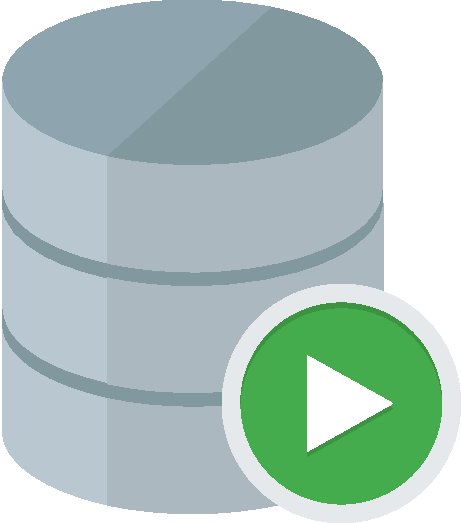
\includegraphics[height=8mm]{images/sec5/oraclesqldeveloper.pdf} \\\textbf{Oracle SQL}\\\textbf{Developer}
} & Oracle SQL Developer est un outil gratuit conçu pour améliorer la productivité et simplifier les tâches de développement des bases de données Oracle. Il s'agit d'un outil graphique entièrement pris en charge pour le développement des bases de données Oracle, y compris le parcours des objets de la base de données, l'exécution des instructions/scripts SQL, la modification et le débogage des instructions PL/SQL. En outre, il est possible d'exécuter un nombre quelconque de rapports fournis, ainsi que de créer et d'enregistrer des rapports personnalisés.\\
{
\includegraphics[height=7mm]{images/sec5/postman.pdf} \\\textbf{Postman}
} & Postman est un environnement de développement d'API complet permettant de concevoir, de mocker, de tester, de surveiller et de publier des API à partir de l'interface utilisateur Postman.\\
{
\includegraphics[height=7mm]{images/sec5/sonarcube.pdf} \\\textbf{SonarQube}
} & SonarQube est une plateforme open source dédiée à l'analyse et à la mesure en continu de la qualité du code source. Elle permet aux développeurs de détecter les bugs et les vulnérabilités ainsi que de réduire les mauvaises pratiques de code, et de ce fait d'améliorer systématiquement la qualité du code. \\
{
\includegraphics[width=7mm]{images/sec5/sourcetree.pdf} \\\textbf{Sourcetree}
} & Développé par Atlassian, SourceTree est un client Git qui intègre très efficacement le workflow Gitflow avec une interface graphique pour gérer presque tout sans avoir à passer par le terminal.\\
{
\includegraphics[height=8mm]{images/sec5/wildfly.pdf} \\\textbf{WildFly}
} & WildFly, anciennement connu sous le nom de JBoss Application Server, est un serveur d'applications open source (LGPL), développé par Redhat, pouvant être utilisé sur tout système d'exploitation fournissant une machine virtuelle Java (JVM). \\
{
\includegraphics[height=4.5mm]{images/sec5/zoom.pdf} \\\textbf{Zoom}
} & La crise sanitaire et la généralisation du télétravail ont largement encouragé l'adoption des outils de visio-conférence. L'un de ces outils est Zoom, qui est essentiellement un outil permettant aux professionnels de mener facilement des visio-conférences et des réunions en ligne, ainsi que d'échanger des messages, des documents, des images, des vidéos et d'autres types de données avec les participants d'un groupe de discussion.\\
\end{longtblr}
\subsubsection{Outils utilisés pour la réalisation de ce rapport}
Adobe Illustrator
Draw.io
LaTeX
Figma
Vs code
\subsection{Démonstration de la fiabilité du nouveau système d'envoi de notifications}
Le traitement par lot, communément appelé Batch dans le jargon informatique, est une problématique très répandue et quasiment incontournable au sein des entreprises et industries qui manipulent d’énormes masses de données. Dans cette section, nous allons vous présenter à travers un exemple d’application, la technologie Spring Batch/Spring Boot permettant de répondre à ce type de besoin.
\subsubsection{Préparation de l'environnement et paramétrage du système}
Afin de préparer la démonstration, nous commencerons par la mise en place de l'environnement d'exécution :
\begin{enumerate}
    \item Établir les données d'entrée : À ce stade, et pour des fins de test, nous allons générer systématiquement quatre fichiers CSV de taille aléatoire. Ces fichiers sont composés de 3 champs :
    \begin{itemize}
        \item \textbf{Le matricule} : valeur numérique servant à identifier le salarié.
        \item \textbf{Le code client} : valeur alphanumérique désignée comme identifiant du client (société).
        \item Le idTech : valeur alphanumérique sert comme identifiant de document.
    \end{itemize}
    \item Créez trois répertoires nommés respectivement "input", "inprogress", et "done".
    \item Déplacez les fichiers CSV préalablement créés vers le répertoire "input" (ou "inprogress") afin de les traiter avec le batcher.
    \begin{figure}[H]
        \centering
        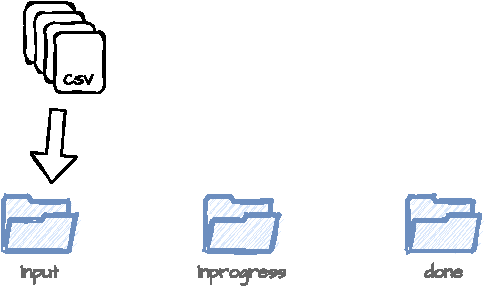
\includegraphics[width=0.45\linewidth]{images/sec5/folders.pdf}
    \end{figure}
    \item Assurer que le fichier properties pointe sur le chemin du repertoire input
\end{enumerate}
L'application réalisée est menée par un fichier de propriétés. ce fichier permet de \dots
parmi les proprité
\subsubsection{Exécution, résultats et interprétation}
\subsubsection{Tests unitaires}
\subsubsection{Audit de code}
\subsubsection{Benchmark}
\subsubsection{Synthèse}
\addcontentsline{toc}{subsection}{Conclusion}
\subsection*{Conclusion}
%%%%%%%%%%%%%%%%%%
